\documentclass{article}

\usepackage{afterpage}
\usepackage{fontspec}
\usepackage{geometry}
\usepackage{hyperref}
\usepackage{lscape}
\usepackage{pgfgantt}
\usepackage{siunitx}
\usepackage{titling}

\title{CRAPS Kernel}
\author{
       Maxime Arthaud
  \and Korantin Auguste
  \and Martin Carton
  \and Étienne Lebrun
  \and Pierre-Louis Michel
}

\begin{document}
  \begin{titlepage}
  \begin{center}
    
\includegraphics[height=1cm]{LogoEnseeiht}\\\vspace{1cm}
    \hrule\vspace{0.5cm}
    \textsc{\Large\thesubtitle}
    \\\vspace{0.5cm}

    \textbf{\huge\thetitle}
    \\\vspace{0.4cm}
    \hrule\vspace{2cm}

    {\large
      Maxime~\textsc{Arthaud}      \\
      Korantin~\textsc{Auguste}    \\
      Martin~\textsc{Carton}       \\
      Étienne~\textsc{Lebrun}
    }

    \vfill
    {\large January -- March 2015}
  \end{center}
\end{titlepage}

  \tableofcontents
  \newpage

  \section{Introduction}
    This project, suggested by Daniel Hagimont, is based on the CRAPS processor
    developed by Jean-Christophe Buisson and used in the first-year CPU
    architecture courses at ENSEEIHT. The goal is to develop an operating
    system that would run on top of that processor.

    The reasons for that project are that before, it was only possible to do a
    little of assembly directly on the processor to see it work, but nothing
    more.  After our project, it should be possible for students to really see
    the layer that goes on top of the CPU in modern computers: the operating
    system. So that the students can really make the link between the processor
    they just built and the computer and underlying operating systems they use
    everyday.

    \paragraph{}
    The system will be as modular as possible, so that students can reuse parts
    of it and implement their own modules.

  \section{Project Overview}
    The objective of the project is to create an operating system, with a
    scheduler running a few tasks. It will also provide functions to display
    text to the user, do input/output to a permanent storage\dots

    For now, having the OS loading programs dynamically is out-of-scope : the
    goal is to have a very simple functional OS.  We will also have to improve
    the CPU to make it support our OS. Specifically we know we will have to
    support the RAM chips that are on the FPGA: currently, we have \SI{2}{kB}
    of RAM that are built in, but that's clearly not enough.

    Another important
    and time-consuming element will be to adapt the compiler we made last year
    during a project, to make it generate the CRAPS assembly. We will
    surely need to make other modifications to the compiler.

  \section{Method, Tools and Test Facilities}
    \subsection{Method and Tools}
    A room and two FPGAs have been made available for us to work.
    The operating system will be written in C, once we have a functional
    compiler.
    At the end, we want to be able to run a few processes that will communicate
    with the user, and store data in permanent memory.

     \subsection{Test Facilities}
    Tests are quite a though point, as our only way to test is to put
    our code on the board and try it. With the given software, it can not be
    done automatically.
    We will explore the feasibility to rewrite the monitor to be able to load
    the assembly code with a command line, which would allow automatization, but
    it could take too much time.
    We will produce test code for the functionalities we choose to implement.

  \section{Software Team Organisation and Responsibilities}
    \begin{itemize}
      \item Korantin Auguste as \textit{developer}
      \item Maxime Arthaud as \textit{tester}
      \item Martin Carton as \textit{project leader}
      \item Étienne Lebrun as \textit{quality manager}
      \item Pierre-Louis Michel as \textit{tester}
    \end{itemize}

  \section{Project Monitoring and Controls}
    A Gantt diagram for the project is available on page \pageref{fig:gantt}.

    Controls: meetings?

    %\afterpage{\newgeometry{top=2cm,bottom=3.5cm}
\begin{landscape}
  \label{fig:gantt}
  \def\pgfcalendarweekdayletter#1{%
    \ifcase#1M\or T\or W\or T\or F\or S\or S\fi%
  }
  \thispagestyle{empty}
  \centering
  \noindent\resizebox{\linewidth}{!}{
    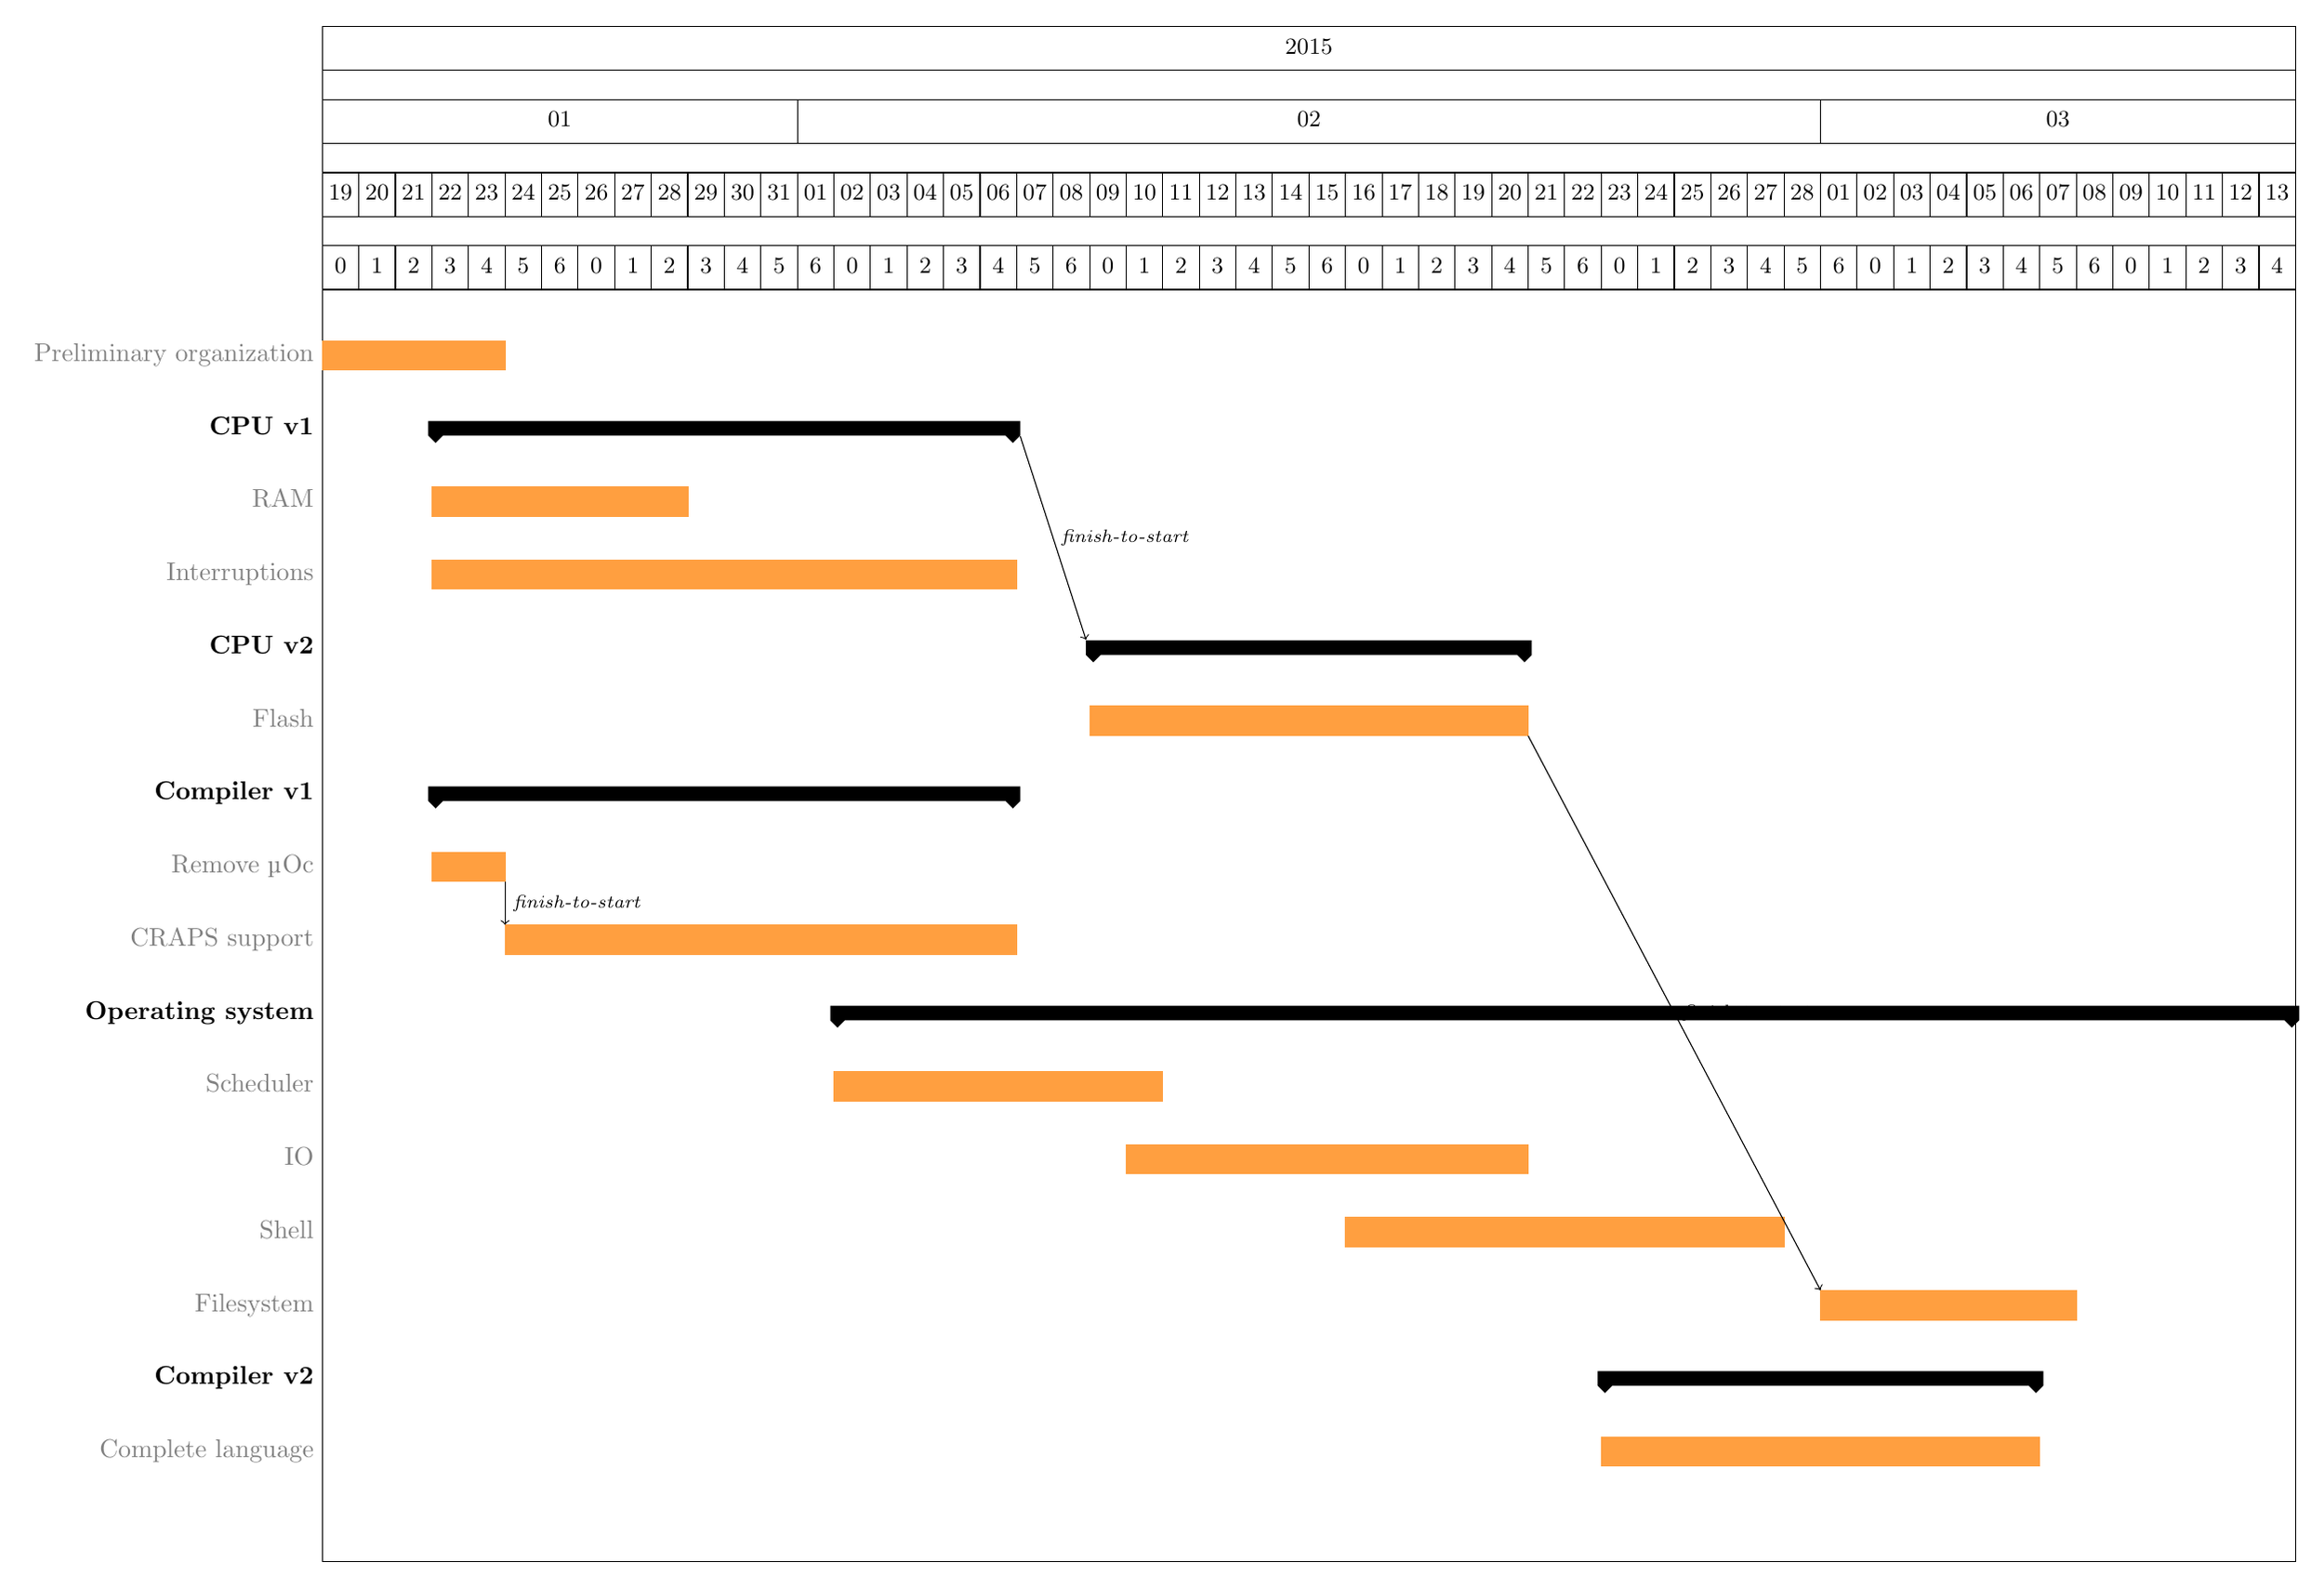
\begin{tikzpicture}
      \begin{ganttchart}[
          /pgf/outer xsep=+0pt,
          bar/.append style={orange!75},
          time slot format=isodate,
          link/.style={->},
          bar label font=\normalsize\color{black!50}
        ]{2015-01-19}{2015-03-13}
        \gantttitlecalendar{year, month, day, weekday=letter}                 \\

        \ganttbar{Preliminary organization}{2015-01-19}{2015-01-23}           \\

        \ganttgroup[name=CPU1]{CPU v1}{2015-01-22}{2015-02-06}                \\
            \ganttbar[name=RAM]{RAM}{2015-01-22}{2015-01-28}                  \\
            \ganttbar[name=IT]{Interruptions}{2015-01-22}{2015-02-06}         \\

        \ganttgroup[name=CPU2]{CPU v2}{2015-02-09}{2015-02-20}                \\
            \ganttlink[link type=f-s]{CPU1}{CPU2}
            \ganttbar[name=flash]{Flash}{2015-02-09}{2015-02-20}              \\

        \ganttgroup[name=comp1]{Compiler v1}{2015-01-22}{2015-02-06}          \\
            \ganttbar[name=MOC]{Remove µOc}{2015-01-22}{2015-01-23}           \\
            \ganttbar[name=CRAPS]{CRAPS support}{2015-01-24}{2015-02-06}      \\

        \ganttgroup[name=os]{Operating system}{2015-02-02}{2015-03-13}        \\
            \ganttbar{Scheduler}{2015-02-02}{2015-02-10}                      \\
            \ganttbar{IO}{2015-02-10}{2015-02-20}                             \\
            \ganttbar{Shell}{2015-02-16}{2015-02-27}                          \\
            \ganttbar[name=FS]{Filesystem}{2015-02-29}{2015-03-07}            \\

            \ganttlink[link type=f-s]{flash}{FS}

        \ganttgroup[name=comp2]{Compiler v2}{2015-02-23}{2015-03-06}          \\
            \ganttbar[name=MOREC]{Complete language}{2015-02-23}{2015-03-06}  \\

            \ganttlink[link type=f-s]{MOC}{CRAPS}
      \end{ganttchart}
    \end{tikzpicture}
  }
\end{landscape}
\restoregeometry
}

  \section{Meetings and reporting}
    Two kinds of meetings are planned:
    \begin{itemize}
        \item a meeting once a week with the client;
        \item a meeting once a week with the industrial supervisor.
    \end{itemize}
    Minutes of these meetings are available is the repository.

    Additionally we regularly meet to talk about the advancement of the project.

  \section{Management of actions}
    A file with the actions (listing who did what and when) has been created.

  \section{Management of risks}
    \begin{itemize}
      \item A FPGA can be damaged, making any test impossible. This is likely to
          happen but we have two FPGAs and the possibility to have more in case
          of problem.
      \item We may not be able to integrate the RAM, leading to huge memory
          limitations that may make the project impossible
    \end{itemize}

  \section{Management of change requests}
    When a change request occurs from the client, we evaluate the additional
    time it may take, in order to decide whether it can be incorporated to the
    delivery and what would be the cost in terms of delay.

  \section{Quality and Configuration management}
    We have decided to use a version control system to record every document and
    all the source code produced. A Git repository has been created on
    Github\footnote{Github repository:
    \url{https://github.com/mcarton/CRAPS-Kernel}}.
    It will contain:
    \begin{itemize}
      \item The source code of our project, for the processor as well as for the
            operating system
      \item The test code we produce according to the software test plan
      \item The documentation, as described in the following section
    \end{itemize}

  \section{Documentation}
    As the system will be modular and expected to be used by students, a
    documentation of every module will be provided.

    \begin{itemize}
      \item User Manual
      \item Modifications of the CRAPS processor
      \item This present Software Development Plan
      \item The specifications
      \item The test plan and test reports
    \end{itemize}

    \section{Deliveries}
      The software will be delivered in several iterations, described in the
      specifications. Each delivery will be accompanied by the corresponding
      documentation.
      Delivery dates:
        TODO

  \newpage
  \begin{appendix}
    \section{Specifications}
      \begin{itemize}
        \item Improvement of the processor
          \begin{itemize}
            \item the FPGA shall have access to the RAM to have more than
              \SI{2}{kB} of memory
            \item the FPGA shall be able to use the \textit{RS-232} serial port
              to communicate with the user
            \item the FPGA shall have a permanent storage, such as flash memory
          \end{itemize}
        \item Compiler
          \begin{itemize}
            \item the compiler shall have a CRAPS backend
            \item the language shall be more similar to C
              \begin{itemize}
                \item operators shall have the same priority
                \item users should be able to use arrays
              \end{itemize}
          \end{itemize}
          \item Development of the OS
            \begin{itemize}
              \item test task 1: make a led blink
              \item test task 2: communicate with the user
                \begin{itemize}
                  \item development of a mini-shell ?
                  \item management of the I/O from the software
                \end{itemize}
              \item scheduler and process management
              \item system calls and API of the OS:
                \begin{itemize}
                  \item very simple file system
                  \item user I/O (using the serial port or other means)
                  \item system task to manage the I/O?
                  \item functions like \verb+malloc+, etc.
                \end{itemize}
            \end{itemize}
        \item Report
          \begin{itemize}
            \item write the developer documentation
          \end{itemize}
      \end{itemize}
  \end{appendix}
\end{document}
